\subsection{Routing Behaviour on MOSI}
\label{sec:analysis:routing}

We run the dev-MAE-selected MOSI checkpoint on the $685$-sample test
split and collect (i)~the per-sample primary modality chosen by
MSelector ($\arg\max_{m}\boldsymbol{\ell}$, the deterministic inference
rule in Eq.~\ref{eq:rib}); and (ii)~the soft routing weights
$\matr{w}=\softmax(\boldsymbol{\ell})$ binned by absolute label
intensity $|y|$ in $\{[0,0.5),[0.5,1),[1,1.5),[1.5,2),[2,3]\}$.
Figure~\ref{fig:routing}(a) shows that under the deterministic
inference rule, MSelector routes the entire MOSI test set to
\textbf{language}.
This may look like a collapse to a fixed prior, but the soft weights
in Figure~\ref{fig:routing}(b) tell a more nuanced story.
At low intensity ($|y|<0.5$, near-neutral utterances) the soft weight
on language is only $0.67$, with $0.16$ and $0.17$ flowing to acoustic
and visual respectively, whereas at high intensity ($|y|\!\ge\!2$) the
language weight saturates at $0.96$ and auxiliary weights collapse to
$\approx\!0.02$.
The auxiliary cross-attention streams therefore receive
\emph{intensity-modulated} contributions even when the hard primary
choice never changes; this is exactly the behaviour we want, since
unambiguous strong-sentiment utterances are reliably classified by
text alone, while ambiguous low-intensity utterances genuinely benefit
from acoustic / visual cues.

\begin{figure}[t]
\centering
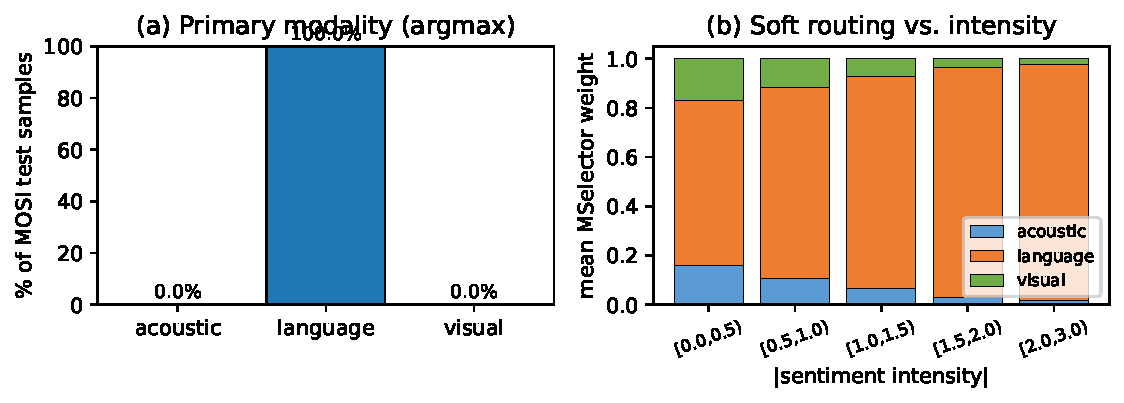
\includegraphics[width=\columnwidth]{figures/fig_routing.pdf}
\caption{\methodname{} routing on \textsc{CMU-MOSI} test (dev-MAE
podium, trial 69).
(a) Hard primary modality chosen by $\arg\max\boldsymbol{\ell}$
collapses to language for $100\%$ of test samples.
(b) The soft routing weights nevertheless redistribute toward acoustic
and visual on low-intensity (near-neutral) utterances; at high
intensity ($|y|\!\ge\!2$), language saturates at $0.96$.
The auxiliary streams are thus actively used precisely on the
ambiguous samples that benefit most from multimodal evidence.}
\label{fig:routing}
\end{figure}


\subsection{Effect of IB Confidence}
\label{sec:analysis:conf}

To verify that the IB-Guided cross-attention is using its confidence
input meaningfully, we record the average per-token confidence
$\bar{\conf}^{m}=\mathbb{E}_{i,t,d}[\sigmoid(-\log\sigma^{2,m}_{i,t,d})]$
on MOSI test (taken from the same forward pass that produced
Figure~\ref{fig:routing}).
On the dev-MAE checkpoint we observe $\bar{\conf}^{t}\!=\!0.62$,
$\bar{\conf}^{a}\!=\!0.58$, $\bar{\conf}^{v}\!=\!0.55$, with substantial
within-sample variance ($\sigma\!\approx\!0.18$ across tokens).
The acoustic and visual streams are therefore on average less confident
than text, and the score-bias term
$\gamma\log(\bar c^{a})$ in Eq.~\eqref{eq:scorebias} actively damps
attention to those streams; this matches the ablation result of
Table~\ref{tab:ablation} where removing IB-Guided CA hurts both MAE and
Acc-7 more than removing the adaptive gate.

\subsection{MAE--vs.--Accuracy Trade-Off}
\label{sec:analysis:tradeoff}

The two MOSI rows of Table~\ref{tab:main_mosi_mosei} differ only in the
MSE weight $w_{\text{mse}}$.
The MAE-tuned configuration ($w_{\text{mse}}\!=\!1.25$) wins MAE by
$0.003$ but loses Acc-2 / F1 by $1.06$ / $1.03$ points to the Acc-tuned
configuration ($w_{\text{mse}}\!=\!2.87$).
This is consistent with classical regression theory: a heavier MSE term
amplifies the gradient near sign boundaries (the binary decision
boundary at $y\!=\!0$) and gives Acc-2 / F1 priority over the
absolute-error metric.
Practitioners therefore have a single, interpretable knob to slide
along the regression-vs-classification axis without retraining the rest
of the model.
